\documentclass[sigconf]{acmart}
% % Packages
\usepackage{soul}
\usepackage{amsmath}
\usepackage{amsfonts}
\usepackage{hyperref}

% Specify path to images
\graphicspath{ {./img/} }


\author{Keanelek Enns}
\email{keanelekenns@uvic.ca}
\affiliation{%
  \institution{University of Victoria}
  \department{Computer Science}
  \streetaddress{PO Box 1700 STN CSC}
  \city{Victoria}
  \state{British Columbia}
  \country{Canada}
  \postcode{V8W 2Y2}
}

\author{Tengkai Yu}
\email{FIXTHIS@uvic.ca}
\affiliation{%
  \institution{University of Victoria}
  \department{Computer Science}
  \streetaddress{PO Box 1700 STN CSC}
  \city{Victoria}
  \state{British Columbia}
  \country{Canada}
  \postcode{V8W 2Y2}
}

\author{Venkatesh Srinivasan}
\email{srinivas@uvic.ca}
\affiliation{%
  \institution{University of Victoria}
  \department{Computer Science}
  \streetaddress{PO Box 1700 STN CSC}
  \city{Victoria}
  \state{British Columbia}
  \country{Canada}
  \postcode{V8W 2Y2}
}

\author{Alex Thomo}
\email{thomo@uvic.ca}
\affiliation{%
  \institution{University of Victoria}
  \department{Computer Science}
  \streetaddress{PO Box 1700 STN CSC}
  \city{Victoria}
  \state{British Columbia}
  \country{Canada}
  \postcode{V8W 2Y2}
}

\title{Explaining Models for Brain Network Classification}

\begin{document}

\begin{abstract}

\end{abstract}

\maketitle

\section{Introduction}

Graph classification, the process of labelling graphs as belonging to certain categories or classes, has applications in many important domains.
This paper will focus on brain network classification, a particularly interesting application of graph classification that can be used to provide insights and diagnoses for neurological disorders such as Autism Spectrum Disorder (ASD).
These insights and diagnoses can further our understanding of such disorders and can aid in providing treatment and support to improve the lives of individuals possessing them.

Machine learning (ML) and artificial intelligence (AI) have been shown to out-perform humans significantly in a multitude of domains \cite{grace2018,fogel2018,brzezicki2020,kahng2021}, and the domain of graph classification is no exception \cite{kong2019}.
But how is performance measured for graph classification?
Metrics such as accuracy, precision, and recall are essential for evaluating any classifier \cite{elkan2012}, and there is no doubt that ML and AI models can achieve impressively high scores in such areas.
However, recently there has been a trend towards \emph{explainability} in the AI world \cite{hassan2021,linardatos2020}.

This is because industries, governments, and organizations, especially those that deal with critical decision making such as the medical field, are hesitant to adopt prediction models without knowing \emph{how and why} they make decisions, regardless of how accurate these models are reported to be \cite{asan2020}.
Therefore, it is increasingly important to find a balance between classification models that are explainable and simple to understand, while also achieving high accuracy, precision, and recall scores.

Another benefit of emphasizing explainability is to provide insights that may not have been detected through classical methods and may lead to further advancements in research.
These insights could be especially helpful to neuroscientists when it comes to studying less understood neurological disorders.

The criteria for diagnosing ASD are vague compared to other neurological disorders \cite{dsm52013}, and even underwent changes within the last decade \cite{grant2013}.
Furthermore, ASD can vary widely in severity.
If black-box ML models alone are to be used for diagnosing ASD in practice, biases of initial models could compound, as diagnoses from such models may inevitably be used as training data for future models.
For such a loosely understood disorder as ASD, this could potentially mutate the practical definition of the disorder or favour certain expressions of it.
Therefore it is critical that such models are highly explainable.
This allows experts to evaluate the biases of the models and provide correction.

In their paper, "Explainable Classification of Brain Networks via Contrast Subgraphs", Lanciano \emph{et al.} proposed a method for translating brain networks into two dimensional vectors with a simple interpretation \cite{lanciano2020}.
This translation of a graph into a more understandable representation is known as a graph embedding and is fundamental to many graph classification problems \cite{goyal2018}.
The graph embedding employed by Lanciano \emph{et al.} involves the use of contrast subgraphs (CSs), which we define later in this paper.

In this study, we sought to reproduce the findings of Lanciano \emph{et al.} as well as discover alternatives or improvements to the methods described in their paper with respect to creating highly explainable and highly performant models \cite{lanciano2020}.
In light of this, we summarize our contributions as follows:

\begin{itemize}
    \item We perform a replication of the novel work done by Lanciano \emph{et al.}
    \item We demonstrate various improvements to the CS method.
    \item We develop a new graph embedding technique named Discriminative Edges (DE) that provides improved accuracy with a fraction of the computational complexity of the CS method, all while maintaining similar explainability.
    \item Taking advantage of the node identity aware (NIA) data, we explore deep learning solutions with neural networks and compare existing explanation strategies with the explanations of the more simplistic methods.
    \item We provide a replication package to recreate all the work done in this study, as well as provide a complete and optimized implementation of Lanciano \emph{et al.}'s graph embedding process.
\end{itemize}

The following section will discuss related work.
Preliminary information about the data sets and notation used for this study will be covered in the section that follows.
We will then describe the CS embedding technique as well as our own embedding technique, DE.
The experiments conducted and the results obtained are outlined in the Experiments section, and finally, we end the paper with discussions and conclusions for this study and suggestions for future research.



\section{Related Work}

% Manuscripts page: http://fcon_1000.projects.nitrc.org/indi/abide/manuscripts.html

Dai and Wang worked on creating explanations that are built into a GNN \cite{dai2021} rather than trying to find an explanation after the GNN had made its classification.
They found their method to be less biased and more computationally efficient when compared to using a post-hoc explainer such as GNN explainer.
However, one problem is that many black box prediction models are already in use by many organizations, so they require a post-hoc solution (find citation for this, I know there is one, just can't remember which one).

Wang \emph{et al.} recently proposed a method, named DHC-E, for embedding graphs in a generalizable way that does not require any hyperparameters \cite{hwang2021}. The embedding has a moderate number of dimensions depending on the graph set analyzed and is based on the h-index values of each vertex in the graph. They used principal component analysis to present the graph embeddings in two dimensions.

In this paper, we are studying a special case of graph classification where all considered graphs possess the same set of vertices.
This concept is called \emph{node identity awareness} (NIA).

Maddalena \emph{et al.} compared NIA graph embedding techniques such as denoising autoencoders (DAE) \cite{gutierrez2019} and a matrix factorization approach named Joint Embedding (JE) \cite{swang2021} for classifying brain networks among other network types, but these embedding techniques were lacking in terms of performance and interpretability \cite{maddalena2021}.

Reli{\'o}n \emph{et al.} worked to identify brain networks of individuals with schizophrenia using convex regularization and selecting important edges and nodes \cite{relion2019}. Although claiming interpretability and explainability as a goal, they do not emphasize or discuss this aspect of their work.

Talk about the shortcomings of the work from lanciano here \cite{lanciano2020}?

Perotti \emph{et al.} created a tool for deriving SHAP values in the domain of graph classification by using motifs as features.
This work focuses on explaining the decisions of black-box classifiers, but determining these explanations is computationally expensive (need to look into how/whether they solved that).

\cite{abbas2020} - Diagnoses with behavioural info.

\cite{thomas2020}
\cite{sewani2020}.

\cite{kong2019}
\cite{perotti2022}
\cite{coupette2022}

SCOTT WILL NEED TO WRITE ABOUT THE NEURAL NETWORK RELATED WORKS. Look at references 25, 26, 38, 42 from Lanciano's paper. Specifically \href{https://ieeexplore.ieee.org/document/8970823}{26} which claims 99\% accuracy with DNN approach.

\section{Preliminaries}
% http://preprocessed-connectomes-project.org/abide/index.html
% Check to see if ABIDE II has also been similarly preprocessed
% https://www.frontiersin.org/10.3389/conf.fninf.2013.09.00041/event_abstract
\textbf{Data.}
The data sets in this paper originated from the Autism Brain Imaging Data Exchange (ABIDE) project \cite{craddock2013} and were processed by Lanciano \emph{et al.}
This processing resulted in groups of simple, undirected, and unweighted graphs (brain networks) defined over a common set of 116 vertices.
The brain networks are labelled with two classes: Typically Developed (TD) or Autism Spectrum Disorder (ASD).

The vertices of the brain networks correspond to regions of interest (ROIs) in the brain, the set of ROIs are common across all the brain networks considered in the data set, thus our graphs exhibit NIA.
The edges of each brain network correspond to functional (as opposed to structural) connections in the brain.

For a more thorough discussion of the data sets used and the processing that was performed by Lanciano \emph{et al.}, please see section 5 of their paper \cite{lanciano2020}.

\textbf{Notation.}
We reuse the notation specified in Lanciano \emph{et al.}'s paper and reiterate the important notation here.

Let the $i^{th}$ brain network be represented as an undirected, unweighted graph $G_i = (V, E_i)$, where $V$ is the common vertex set representing the 116 ROIs of the brain as discussed previously (i.e. $|V| = 116$) and $E_i$ is the set of edges belonging to $G_i$ (note: $E_i \subset V \times V$).

Let a \emph{summary graph} corresponding to a set of brain networks $\mathcal{A}$ be a weighted, undirected graph $G^{\mathcal{A}} = (V, w^{\mathcal{A}})$, where $w^{\mathcal{A}}: V \times V \rightarrow \mathbb{R}_+$ is a weight function that assigns a value to each pair of vertices in $V$.
For vertices $u,v \in V$, we define $w^{\mathcal{A}}(u,v)$ to be the fraction of networks in $\mathcal{A}$ that contain the edge $(u,v)$.

\section{Contrast Subgraphs} \label{cs}

A contrast subgraph is defined as a subset of vertices that induces a dense subgraph in one graph and a sparse subgraph in another, assuming that the graphs share a common vertex set.
We echo the problem definition of finding contrast subgraphs from the work of Lanciano \emph{et al.}

\emph{Problem 1 (Contrast Subgraph). Given two sets of observation graphs, i.e. the condition group $\mathcal{A} = \{G^{\mathcal{A}}_1, . . . , G^{\mathcal{A}}_{|\mathcal{A}|}\}$ and the control group $\mathcal{B} = \{G^{\mathcal{B}}_1, . . . , G^{\mathcal{B}}_{|\mathcal{B}|}\}$, and corresponding summary graphs $G^{\mathcal{A}} = (V, w^{\mathcal{A}})$ and $G^{\mathcal{B}} = (V, w^{\mathcal{B}})$, we seek to find a subset of vertices $S^* \subseteq V$ that maximizes the contrast subgraph objective}
\begin{align*}
    \delta (S) = \sum_{u,v \in S} \left(w^{\mathcal{A}}(u,v) - w^{\mathcal{B}}(u,v) - \alpha\right)
\end{align*}
\emph{where $\alpha \in \mathbb{R}_+$ is a user-defined parameter.}

Their paper also defines a symmetric variant of the contrast subgraph problem (\emph{Problem 2}) which shares the same definition of \emph{Problem 1}, but with an alternative objective

\begin{align*}
    \sigma (S) = \sum_{u,v \in S} \left(|w^{\mathcal{A}}(u,v) - w^{\mathcal{B}}(u,v)| - \alpha\right)
\end{align*}

The parameter $\alpha$ is used to penalize large contrast subgraphs.
It can be adjusted to vary the proportion of edges that are considered detrimental to the contrast subgraph objective.

These problems can be simplified to finding a set of vertices that induce a dense subgraph in the difference of the two summary graphs.
Consider the difference network  $G^{\mathcal{A} - \mathcal{B}} = (V, w^{\mathcal{A} - \mathcal{B}})$, where \\ $w^{\mathcal{A} - \mathcal{B}}(u,v) = w^{\mathcal{A}}(u,v) - w^{\mathcal{B}}(u,v), \forall u,v \in V$.
In this context, finding a contrast subgraph is equivalent to finding a dense subgraph in the difference network.
There are many notions of density studied in the literature.
Lanciano \emph{et al.} base the constrast subgraph objective off of the optimal quasi-clique problem \cite{tsourakakis2013}.

Note that contrast subgraphs themselves do not constitute a graph embedding technique, but they can be used in the following ways to embed a graph.

\textbf{Problem 1.}
Lanciano \emph{et al.} use contrast sugbraph overlap to create two features for each brain network.
Because the problem is asymmetric, two contrast subgraphs are needed.
One is found in the difference network $G^{TD - ASD}$ (which is the result of subtracting the summary graph $G^{TD}$ from the summary graph $G^{ASD}$) and the other is found in $G^{ASD - TD}$.
Each feature of a brain network's embedding corresponds to the number of edges in common between the brain network and each contrast subgraph.
% Maybe this image should be displayed in the experiments section, but alluded to here
Figure \ref{fig:prob1} positions some of the brain networks in two dimensions based on their embeddings for problem 1. 

\begin{figure}
    \centering
    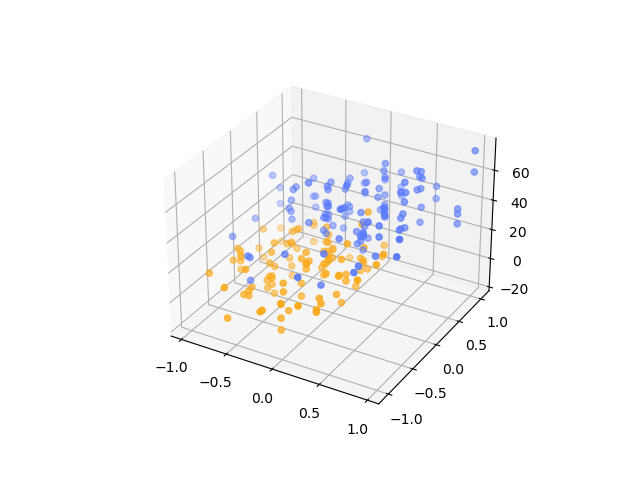
\includegraphics[width=\columnwidth, keepaspectratio=true]{test.png}
    \caption{Show a representative plot for problem 1}
    \label{fig:prob1}
\end{figure}

\textbf{Problem 2.}
A single contrast subgraph is found in the difference network containing absolute valued edge weights (i.e. $|G^{TD - ASD}|$).
The contrast subgraph is used to induce subgraphs in both of the summary graphs (i.e. $G^{TD}$ and $G^{ASD}$) as well as each individual brain network.
The distances, computed as the $L_1$ norms, from the induced brain network to each summary graph are then used as the two features for this embedding.
% Maybe this image should be displayed in the experiments section, but alluded to here
Figure \ref{fig:prob2} positions some of the brain networks in two dimensions based on their embeddings for problem 2. 

\begin{figure}
    \centering
    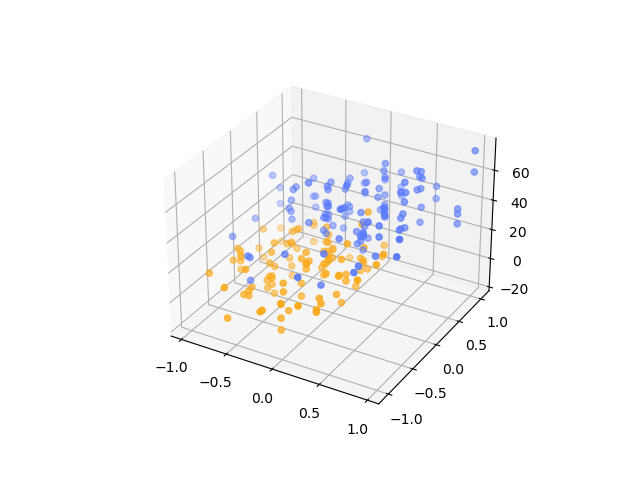
\includegraphics[width=\columnwidth, keepaspectratio=true]{test.png}
    \caption{Show a representative plot for problem 2}
    \label{fig:prob2}
\end{figure}




\subsection{Improvements} \label{improvements}

Based on our experiments, the original contrast subgraph embedding techniques are quite slow, and their accuracies are not far above the baseline accuracy (i.e. the accuracy obtained when the most dominant class is always predicted).
Therefore we turned our attention to developing improvements for the contrast subgraph embedding technique.

\textbf{Quadratic Programming.}
We looked further into the work by Cadena \emph{et al.} which was repurposed by Lanciano \emph{et al.}
When creating a mathematical problem formulation for finding a dense subgraph in a signed network, Cadena \emph{et al.} proposed a quadratic programming problem.
In their study, they chose to approximate the quadratic program with a semidefinite program and a rounding technique \cite{cadena2016}.
Lanciano \emph{et al.} then used this implementation to find a contrast subgraph in their context.

However, because the goal is to find a dense subgraph in a small difference network (116 by 116), it seemed reasonable to implement a QP solver to solve the problem directly.
We used a Python library named CVXOPT\footnote{This library can be found at \url{https://cvxopt.org/}}.
None of the QP solver libraries we found were able to restrict potential solution vectors to discrete values such as \{-1,1\} (i.e. out or in), so we restricted solution values to [-1,1] rounding positive values to 1 and non-positive values to -1.

% TODO: I STILL NEED TO CALCULATE THIS!!!
The speed increase that resulted from changing the solver was significant as we will discuss in the experiments section.

\textbf{Local Search Optimization.}
The QP and SDP solvers only approximate the densest subgraph, so a local search step is used to improve the density of the chosen subgraph.
The localSearch algorithm developed by Tsourakakis \emph{et al.} and used by both Cadena \emph{et al.} and Lanciano \emph{et al.} works by considering the density of the subgraph if each vertex outside the subgraph were to be added to the subgraph, adding them when it increases the density.
This is repeated until all the vertices have been considered.
Afterwards, the algorithm seeks to remove a single vertex from the subgraph and does so if it finds one that increases the density.
This process is then repeated until a maximum number of iterations have been reached, or no vertices can be added or taken away from the subgraph to increase its density.
The pseudocode for the original algorithm can be found in their paper \cite{tsourakakis2013}.

Considering the goal of the local search algorithm is to increase the density of the subgraph, we made a modification to the algorithm such that it attempts to remove as many vertices as it can in each iteration (removing them only if they increase the density).
This modified local search algorithm can be seen in the replication package for this study, and was found to increase the accuracy of the classifiers that used it over the original implementation.

\textbf{Top-k Contrast Subgraphs.}
Finally, we follow Lanciano \emph{et al.}'s suggestion for future work and use the top-k contrast subgraphs.
We did not implement it according to the suggested method \cite{balalau2015}, but instead took the approach described by Tsourakakis \emph{et al.} in section 4.1 of their paper \cite{tsourakakis2013}.
We removed the vertices of each contrast subgraph as it was found and searched for a new contrast subgraph among the remaining vertices of the graph until all $k$ contrast subgraphs had been found.

The resulting $k$ embeddings for each new brain network were added together feature-wise to obtain the final embedding.



\section{Discriminative Edges}
In section 5.1 of Lanciano \emph{et al.}'s paper, it was shown that the degrees of each vertex in the studied brain networks did not vary significantly between the two classes \cite{lanciano2020}, yet the contrast subgraphs are defined as a set of vertices, and every edge induced by these vertices is used for classification.
In light of this, we thought it would be beneficial to consider only the \emph{edges} that are important for distinguishing between the classes.

The discriminative edges (DE) embedding technique employs a very simple computation for calculating the similarity of a new brain network with each of the two summary graphs.
Initially, the idea was to identify the $n$ most positive edges and the $n$ most negative edges in the difference network $G^{ASD - TD}$.
These are the edges with the greatest disparity between the two classes (positive edges are more common in ASD brain networks, and negative edges are more common in TD brain networks), and are thus, the most discriminative edges.

For each new brain network $G_i$, we calculate the dot product of the n most positive edges in $G^{ASD - TD}$ with the corresponding edges of $G_i$ (in this case, $G_i$ is unweighted, so present edges have a value of 1, and edges that are not present have a value of 0, however, this calculation would still be effective if $G_i$ were weighted).
This gives $G_i$'s similarity with the ASD class.
A similar calculation is done for the negative edges to give the similarity with the TD class.
These similarities are used as the two features of the technique.

With this incredibly simple algorithm, we achieved results that were very similar to those obtained from the contrast subgraph technique.
However, with further improvements, DE managed to surpass the performance of the contrast subgraph technique while remaining computationally efficient and easy to understand.

Rather than ignoring the values of edges in the difference network corresponding to edges that do not exist in $G_i$, we made use of this information by scaling the edge values of $G_i$ such that nonexistent edges have a value of -1 and present edges continue to have a value of 1 (this scaling can also be applied in the case where $G_i$ is weighted).
This means that not having an edge among the most discriminative edges actually counts against the similarity score for each case.

Finally, we added a third feature to the embedding technique.
This feature is derived in a very similar way, but uses every edge in the calculation, and thereby captures more information.
It is calculated by scaling the edge values of $G_i$ as discussed previously, multiplying each edge to its corresponding edge in the difference network, and summing the values.
This gives one score, a positive value implies similarity with the ASD class, whereas a negative value implies similarity with the TD class.
% Note that we may need to change the order I mentioned here depending on what the figures show in terms of positive and negative scores \ref{fig:DE}

The DE embeddings encode more information than the contrast subgraph embeddings, they are more efficient to compute, and they are still easy to visualize in three dimensions.



\section{Experiments}

The data used for this study was briefly described in the preliminaries section.
Table \ref{tab:datasets} is a recreation of Table 1 in Lanciano \emph{et al.}'s paper and gives information regarding the logical grouping of the studied individuals.
This will give context for the experiments presented in this section.

\begin{table}%[]
    \centering
    \caption{An overview of the datasets used. The names of each dataset (first column) are indicative of the common traits of the subjects. This grouping was used to limit the impact of confounding factors in the study. The last two columns give the number of subjects belonging to the TD and ASD classes respectively.}
    \begin{tabular}{c c c c}
        \hline
        Dataset & Description & TD & ASD \\
        \hline
        children &  Age $\leq$ 9 & 52 & 49 \\
        adolescents &  Age $\in [15,20]$ & 121 & 116 \\
        eyesclosed &  Eyes closed during scanning & 158 & 136 \\
        male &  Male individuals & 418 & 420 \\
        \hline
    \end{tabular}
    \label{tab:datasets}
\end{table}

\subsection{Replication}

We began our experiments with an attempt to replicate the results of Lanciano \emph{et al.} using the replication package provided (links to their repository and our repository can be found in appendix \ref{artifacts}).
However, unfortunately, no code was provided (by the time of writing) for evaluating the classifier as discussed in section 5.1 of the original paper.
Furthermore, the code that was present for extracting a contrast subgraph was not conducive to large scale experiments.

With this knowledge, we decided to first rewrite and optimize the existing code such that it could be run repeatedly for our experiments.

The most notable inefficiency was the writing and reading of multiple files and the use of subprocess calls to multiple scripts written in Python and Matlab.
We replaced the Matlab SDP solver, which was reused from the work of Cadena \emph{et al.} \cite{cadena2016}, with a Python implementation using the CVXPY library\footnote{This library can be found at \url{https://www.cvxpy.org/}.}.
The solvers were tested to ensure that the same inputs produced the same outputs (so as to prevent any logical changes from this optimization).

Rather than passing data through the writing and reading of files and the use of subprocess calls to run new scripts, we modified the scripts to directly accept such data as arguments.
We then upgraded the code from Python 2.7 to 3.8 as well as removed unnecessary libraries.
After these changes, we obtained a logically equivalent implementation of the original code with increased computational efficiency.

However, only finding CSs does not constitute a graph embedding technique.
These CSs must be used to translate a brain network into a vector or point.
Because this translation was not present in the repository, we also created the necessary components for the embedding such as inducing subgraphs, counting overlap between contrast subgraphs and new brain networks, and calculating the $L_1$ norm as indicated by the original paper.

Though many components of the original scripts were modified, it is worth noting that many components were reused, and the modifications were tested to ensure logical equivalency.
After this, we developed a module for evaluating the embedding technique using five-fold cross validation.

We then ran our experiments using the alpha parameters reported by Lanciano \emph{et al.}, but the resulting constrast subgraphs were completely empty due to alpha being too large.
Later in our experiments, the authors released a clarification that the reported values were percentiles, not alpha values.
These percentiles correspond to the ratio of edges that are shifted to be considered detrimental to the CS objective (e.g. a percentile value of 70 indicates that we should shift the edge weights down such that only the heaviest 30\% of the edges retain a positive edge weight).
At this point, we had already tuned alpha for their technique, but we returned to test the percentile values reported.
Unfortunately, the results did not agree with what they reported, and our tuning was more beneficial to their technique.

\subsection{Evaluation} \label{evaluation}

To ensure all techniques were evaluated fairly, we developed a common module to run the cross validation tests.
This required that each embedding technique conformed to a common interface:

\begin{itemize}
    \item \textbf{Inputs:} Training graphs, training labels, testing graphs, and any parameters specific to the embedding technique.
    \item \textbf{Outputs:} Training points and testing points (the results of translating each brain network into a point/vector).
\end{itemize}

The testing module takes care of splitting the brain networks into training and testing sets.
After receiving the embedded graphs as points, it shifts the points such that the mean value of each dimension becomes zero, and it scales the points such that a standard deviation is one unit.

The training points are then used to train a classifier, and the classifier is used to predict the class labels of the testing points.
Note that Lanciano \emph{et al.} do not specify what classifier they used for predicting the graph labels of their embedded graphs.
We therefore used the \href{https://scikit-learn.org/stable/modules/generated/sklearn.svm.LinearSVC.html}{LinearSVC classifier} provided by the popular sklearn library as a common choice for all techniques to ensure fairness.

Each iteration of the cross validation routine generates three plots with the following information:
\begin{enumerate}
    \item Training points according to their class labels.
    \item Test points according to their class labels.
    \item Test points according to the predictions that are made.
\end{enumerate}
Furthermore, the number of folds to use is configurable, and there is an option to perform leave-one-out cross validation.
Finally, a cumulative confusion matrix is derived as the sum of the confusion matrices in each of the cross validation iterations and used to calculate the classifier's average accuracy, precision, recall, and f-1 score.

\subsection{Results} \label{results}

After performing the replication of Lanciano \emph{et al.}'s paper to the best of our abilities, we obtained significantly lower accuracies than those reported in Table 2 of their paper.
We performed three rounds of five fold cross validation using the reported parameter values. We briefly report the averaged replication results with their standard deviations in table \ref{tab:replication}.

We were able to produce better results than this with our own parameter tuning, but in either case, the accuracies are well below those reported in Lanciano \emph{et al.}'s work.

\begin{table*}[t]
    \centering
    \caption{Replication results. This is modelled after Table 2 in Lanciano \emph{et al.}'s paper and reports average accuracies with their relative standard deviation.}
    \begin{tabular}{c c c c c}
        \hline
          & Children & Adolescents & EyesClosed & Male\\
        CS-P1 & 0.49 $\pm$ 0.01 & 0.53 $\pm$ 0.01 & 0.49 $\pm$ 0.01 & 0.58 $\pm$ 0.02\\
        CS-P2 & 0.58 $\pm$ 0.03 & 0.54 $\pm$ 0.01 & 0.56 $\pm$ 0.00 & 0.60 $\pm$ 0.00\\
        \hline
    \end{tabular}
    \label{tab:replication}
\end{table*}

Numerous empirical experiments were conducted during the course of this study.
However, due to the computation time required to evaluate our recreation of Lanciano \emph{et al.}'s method, it was not possible to compare results of more rigorous experiments (such as leave-one-out cross validation) for all methods.

Table \ref{tab:results} summarizes the results of the fourth round of experiments.
No tuning was performed in this round, however, tuning from the previous rounds was used to select the best parameter values for each method.
Five fold cross validation was performed for each method on each data set with an 80:20 train to test ratio.

To see the full results of all the experiment rounds and the parameters used, see the \emph{experiments} directory in this paper's repository (found in appendix \ref{artifacts}) as well as the \emph{Replication} directory within it for the replication results previously mentioned.

\begin{table*}[t]
    \centering
    \caption{Classifier Results. CS-SDP refers to our replication of Lanciano \emph{et al.}'s method (with associated P1 and P2 variations). CS-QP refers to our method with all mentioned improvements (QP solver, top-k CSs, and improved local search). DE refers to Discriminative edges. The baseline accuracy represents the accuracy of a classifier that always predicts the most common class in the data set.}
    \begin{tabular}{c c c c c c c}
        \hline
        Dataset & Embedding Technique & Runtime (seconds) & Accuracy (\%) & Precision (\%) & Recall (\%) & F1-Score (\%)\\
        \hline
        children & CS-SDP-P1 & 201.9 & 61.39 & 69.23 & 61.02 & 64.86 \\
        baseline accuracy = 51.49\% & CS-SDP-P2 & 22.3 & 56.44 & 69.23 & 56.25 & 62.07 \\
        & CS-QP-P1 & 7.4 & \textbf{70.30} & \textbf{76.92} & \textbf{68.97} & \textbf{72.73} \\
        & CS-QP-P2 & 4.2 & 65.34 & 73.08 & 64.41 & 68.47 \\
        & DE & \textbf{3.9} & 62.38 & 75.00 & 60.94 & 67.24 \\
        \hline
        adolescents & CS-SDP-P1 & 128.8 & 58.65 & 60.33 & 59.35 & 59.84 \\
        baseline accuracy = 51.05\% & CS-SDP-P2 & 26.2 & 58.65 & 57.02 & 60.00 & 58.47 \\
        & CS-QP-P1 & 9.1 & 61.60 & 66.12 & 61.54 & 63.75 \\
        & CS-QP-P2 & \textbf{5.1} & 63.71 & 66.94 & 63.78 & 65.32 \\
        & DE & 5.8 & \textbf{64.56} & \textbf{70.25} & \textbf{63.91} & \textbf{66.93} \\
        \hline
        eyesclosed & CS-SDP-P1 & 51.3 & 52.38 & 56.33 & 55.63 & 55.97 \\
        baseline accuracy = 53.74\% & CS-SDP-P2 & 16.3 & 58.50 & \textbf{67.09} & 60.23 & 63.47 \\
        & CS-QP-P1 & 12.6 & 60.54 & 65.82 & 62.65 & 64.20 \\
        & CS-QP-P2 & \textbf{5.4} & 58.50 & \textbf{67.09} & 60.23 & 63.47 \\
        & DE & 6.6 & \textbf{60.88} & 65.82 & \textbf{63.03} & \textbf{64.40} \\
        \hline
        male & CS-SDP-P1 & 238.2 & 51.43 & 46.17 & 51.47 & 48.68 \\
        baseline accuracy = 50.12\% & CS-SDP-P2 & 18.3 & 61.81 & \textbf{66.27} & 60.75 & 63.39 \\
        & CS-QP-P1 & 24.4 & 59.90 & 59.57 & 59.86 & 59.71 \\
        & CS-QP-P2 & \textbf{10.4} & 61.81 & \textbf{66.27} & 60.75 & 63.39 \\
        & DE & 14.8 & \textbf{63.01} & 64.59 & \textbf{62.5} & \textbf{63.53} \\
        \hline
    \end{tabular}
    \label{tab:results}
\end{table*}

Clearly our methods show improved efficiency with respect to run time.
It is worth noting, however, that there are odd discrepancies when comparing the run times based on the sizes of the data sets.
This may indicate some inaccuracies due to caching during our experiments.
Still, the results indicate our methods achieve a clear and consistent improvement in efficiency.

The results also indicate a clear and consistent improvement in terms of accuracy, precision, and recall, albeit with a less significant difference.


\section{Discussion}\label{discussion}
\textbf{Discussion of Node-Identity Awareness and its importance with respect to how we treat the data. We do not need to treat it strictly like a graph as lanciano et al do.}

More often than using brain scans, practitioners use behavioural information to diagnose ASD \cite{lord2006, johnson2007, dsm52013}.
In fact, there are even widely used AI based solutions for diagnosing ASD based on behaviourat information \cite{knopf2021}.
% Look at the references of https://www.webmd.com/brain/autism/how-do-doctors-diagnose-autism
If we wish to ensure the accuracy of AI models when providing diagnoses, it would make sense to include such behavioural information in addition to neurological information to train and build models.

Considering ASD is a spectrum, and can affect individuals at very different levels, it might not make sense to view this as a binary classification problem.
Instead, it could be beneficial to break the disorder into multiple additional categories to prevent the biases of ML models from favouring certain expressions of ASD.

Lanciano \emph{et al.} showed that the degrees of each vertex in the studied brain networks did not vary significantly between the two classes \cite{lanciano2020},
yet the contrast subgraphs are defined as a set of vertices, and every edge induced by these vertices is used for classification.
Instead, we should look solely at edges that are important for distinguishing between the classes.

The discriminative edge method considers the most important edges in each class (defined as having the most positive and most negative weights in the difference network) when creating an embedding.
Additionally, it considers the brain network as a whole in its third dimension, which likely captures more interesting information with respect to complex connections in the brain.
However, it does not specifically identify higher order structures in the brain networks that may be leading to the DNN's success.

It was observed in a number of experiments that the local search algorithm would find a subgraph that was significantly different than (sometimes entirely disjoint from) the subgraph found by the SDP solver despite using the SDP solver's solution as a starting point.
This seems to imply that the local search algorithm may have done most of the work in finding the densest subgraph, and that the SDP solving step may have been extraneous, though further investigation would be required to verify this.

\subsection{Limitations and Threats to Validity.}
This study was limited primarily by the data set used.
In many machine learning applications, a large volume of data is needed to adequately train and test new models.
With a small data set, it is difficult to know how generalizable any of the discussed methods are to new brain networks that we wish to classify.
Additionally, the way the data set was created and the individuals that were studied have a large impact on the validity of the classification methods developed.
Elkan gave a helpful discussion of potential pitfalls regarding evaluating classifiers and the way data is gathered \cite{elkan2012}.
In this case, the limitations in data set size and quantity are due to the costly nature of creating such brain networks as individuals need to undergo a series of scans and time series of these scans are used to create the resultant brain network \cite{lanciano2020}.
Furthermore, the ratio of the studied classes is imbalanced when compared to the true ratio of individuals with ASD.

Autism Spectrum Disorder is a very complex disorder with unclear definitions, and it may manifest in various different ways.
Above all this, the brain is a highly complex organ that is not fully understood.
The brains of individuals are unique and develop in complex manners.
There may be a plethora of confounding factors that have an effect on the classification of such networks with respect to identifying ASD in individuals.







\section{Conclusion}



\subsection{Future Work}
\begin{itemize}
    \item Develop classifiers using behavioural and neurological information together.
    \item Consider spaciality of ROIs. \cite{relion2019} suggests this would not be as helpful when the brain network has few ROIs, which is the case with the ABIDE dataset.
    \item Consider different preprocessing of ABIDE dataset.
    \item Run experiments with ABIDE II (if we don't get to it)
    \item Combine brain scan information with behavioural assesment information.
    \item Run simplified classifier alongside black box classifier, and report on the instances when they disagree.
\end{itemize}

Future work should attempt to identify higher order structures (such as triangles, k-clusters, or graphlets of varying size and shapes) as a means of embedding.
This could be done by identifying prominent structures in each summary graph (perhaps after thresholding the edge weights), eliminating structures common to both, and counting the number of overlapping structures that a new brain network has in common with each class.
The challenge associated with this technique comes with the computational complexity of enumerating such high order structures.

As discussed in section \ref{discussion}, this study should be replicated on additional data sets to further test its validity.


\appendix

\section{Artifacts} \label{artifacts}

Lanciano \emph{et al.}'s replication package can be found at \url{https://github.com/tlancian/contrast-subgraph} and was first accessed in January 2022.

Our replication package can be found at \url{https://github.com/keanelekenns/brain-network-classification}.

% References and End of Paper
% These lines must be placed at the end of your paper
\bibliographystyle{ACM-Reference-Format}
\bibliography{refs.bib}
\end{document}
